\documentclass[12pt, a4paper]{article}

\usepackage[margin=2.5cm]{geometry}
\usepackage{graphicx}
\usepackage{amsmath}
\usepackage{amssymb}
\usepackage{booktabs}
\usepackage{hyperref}
\usepackage{listings}
\usepackage{xcolor}
\usepackage{caption}
\usepackage{subcaption}
\usepackage{parskip}
\usepackage{titlesec}
\usepackage{fancyhdr}

\hypersetup{
    colorlinks=true,
    linkcolor=blue!60!black,
    urlcolor=blue!60!black,
}

\lstset{
    language=Python,
    basicstyle=\ttfamily\small,
    keywordstyle=\color{blue!70!black}\bfseries,
    commentstyle=\color{gray},
    stringstyle=\color{orange!80!black},
    breaklines=true,
    frame=single,
    backgroundcolor=\color{gray!8},
    numbers=left,
    numberstyle=\tiny\color{gray},
    xleftmargin=1.5em,
    framexleftmargin=1.5em,
}

\pagestyle{fancy}
\fancyhf{}
\rhead{Collective Robotics -- Tutorial 3}
\lhead{Gandhi, Machida}
\cfoot{\thepage}

\title{
    \vspace{-1cm}
    \textbf{Collective Robotics -- Tutorial 3}\\[0.3em]
    \large Robot Behaviors and Swarm Systems\\[0.5em]
    \normalsize Hochschule Bonn-Rhein-Sieg\\
    Prof.\ Dr.\ Javad Ghofrani
}
\author{Bhavesh Gandhi \and Jaqueline Machida}
\date{31.05.2026}

\begin{document}

\maketitle
\thispagestyle{fancy}
\tableofcontents
\newpage

% =============================================================================
\section{Task 1 -- Buffon's Needle Simulation}
% =============================================================================

\subsection{Overview}

We implement and analyze Buffon's Needle, a Monte Carlo experiment
that estimates the probability that a randomly dropped needle crosses one of a
set of parallel lines and, from that probability, estimates $\pi$.  All
experiments use a needle of length $L = 0.7$ and line spacing $D = 1.0$.  Each
drop is characterized by two random variables: the distance $x$ from the
needle's center to the nearest line and the acute angle $\theta$ between the
needle and the lines.  Source code and plots live under \texttt{Task~1/}.

\subsection{Subtask a -- Derivation of the Crossing Probability}

Because only the position of the needle relative to the nearest line
matters, the sample space collapses to the rectangle $x \in [0, D/2]$,
$\theta \in [0, \pi/2]$, and $x$, $\theta$ are sampled uniformly on it.  The
total sample-space area is therefore
\[
    A_{\text{total}} = \frac{D}{2} \cdot \frac{\pi}{2} = \frac{D\pi}{4}.
\]
A crossing occurs when the vertical projection from the needle's center to
its tip reaches the nearest line, i.e.\ $x \le \tfrac{L}{2}\sin\theta$.
Integrating the crossing condition over $\theta$ gives
\[
    A_{\text{success}} = \int_0^{\pi/2} \frac{L}{2}\sin\theta\, d\theta
    = \frac{L}{2},
\]
so the theoretical crossing probability is
\[
    P = \frac{A_{\text{success}}}{A_{\text{total}}} = \frac{2L}{D\pi}.
\]
Rearranging yields the Monte Carlo estimator for $\pi$:
\[
    \pi \approx \frac{2L\,n}{D\,C},
\]
where $n$ is the number of needle drops and $C$ is the number of observed
crossings.  For $L = 0.7$, $D = 1.0$ the theoretical probability is
$P_{\text{true}} = 1.4/\pi \approx 0.4456$.

\subsection{Subtask b -- Single Simulation ($n = 1000$)}

We sample $n = 1000$ needles by drawing $x \sim \mathcal{U}[0, D/2]$ and
$\theta \sim \mathcal{U}[0, \pi/2]$ independently and applying the crossing
condition.  Figure~\ref{fig:task1-needles} shows one such run, where red
needles correspond to crossings and blue needles to misses.

\begin{figure}[h]
    \centering
    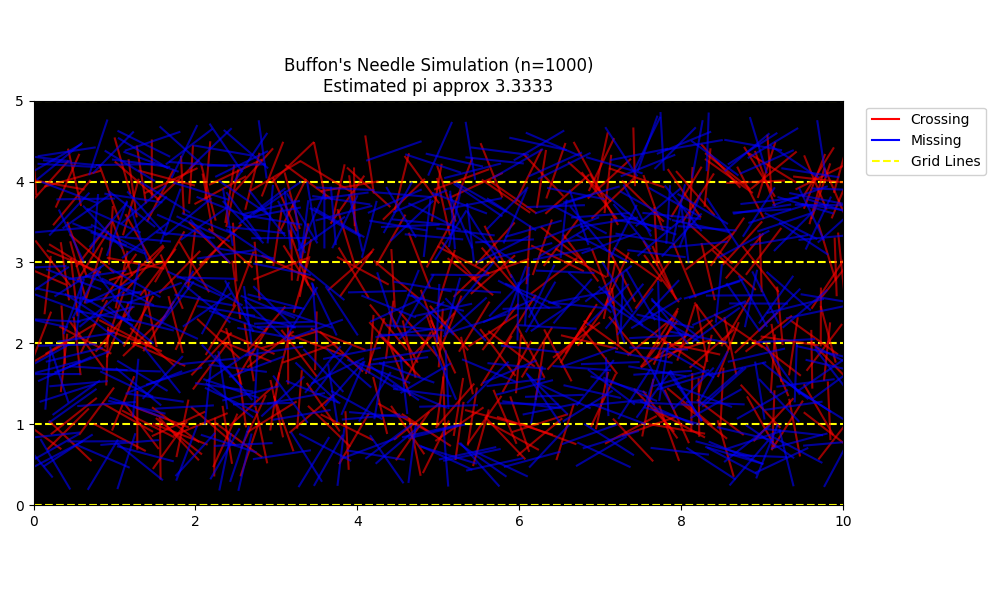
\includegraphics[width=0.7\textwidth]{Task 1/plots/1b_buffon_needle_simulation.png}
    \caption{Single Buffon's Needle simulation with $n = 1000$ drops.
             Red: crossings; blue: misses.}
    \label{fig:task1-needles}
\end{figure}

In the plotted run the estimated $\pi$ is approximately $3.3333$, higher than
the true value $\pi \approx 3.1416$.  This deviation is expected for a single
finite Monte Carlo run: since $\pi$ is estimated as $2Ln/(DC)$, a small
shortfall in the number of crossings produces a noticeably high $\pi$
estimate.

\subsection{Subtask c -- Standard Deviation vs.\ Number of Trials}

To quantify variability we repeat the experiment for each
$n \in \{10, 20, \ldots, 1000\}$ and report the standard deviation of the
estimated crossing probability (Figure~\ref{fig:task1-std}).

\begin{figure}[h]
    \centering
    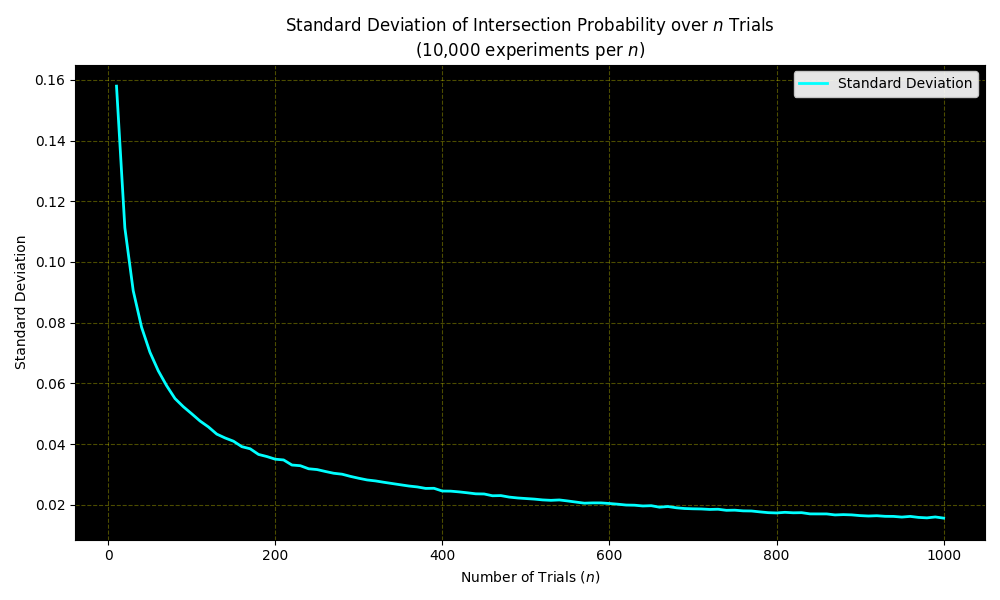
\includegraphics[width=0.7\textwidth]{Task 1/plots/1c_std_dev_vs_n.png}
    \caption{Standard deviation of the estimated crossing probability as a
             function of the number of trials $n$.}
    \label{fig:task1-std}
\end{figure}

The curve starts near $0.16$ at $n = 10$, drops sharply, and flattens to about
$0.015$ by $n = 1000$.  This follows the expected scaling of a binomial
proportion,
\[
    \sigma_{\hat P} = \sqrt{\frac{P(1-P)}{n}},
\]
i.e.\ uncertainty shrinks like $1/\sqrt{n}$.  Returns therefore diminish: the
first few hundred trials buy most of the precision and later trials buy
proportionally less.

\subsection{Subtask d -- Probability Convergence with 95\,\% CI}

For a measured proportion $\hat P$ after $n$ trials, the binomial 95\,\%
confidence interval is
\[
    \hat P \pm 1.96\sqrt{\frac{\hat P(1-\hat P)}{n}}.
\]
We run 50 independent experiments up to $n = 100$ and plot the running
probability estimate of each one together with the CI envelope around
$P_{\text{true}}$ (Figure~\ref{fig:task1-conv}).

\begin{figure}[h]
    \centering
    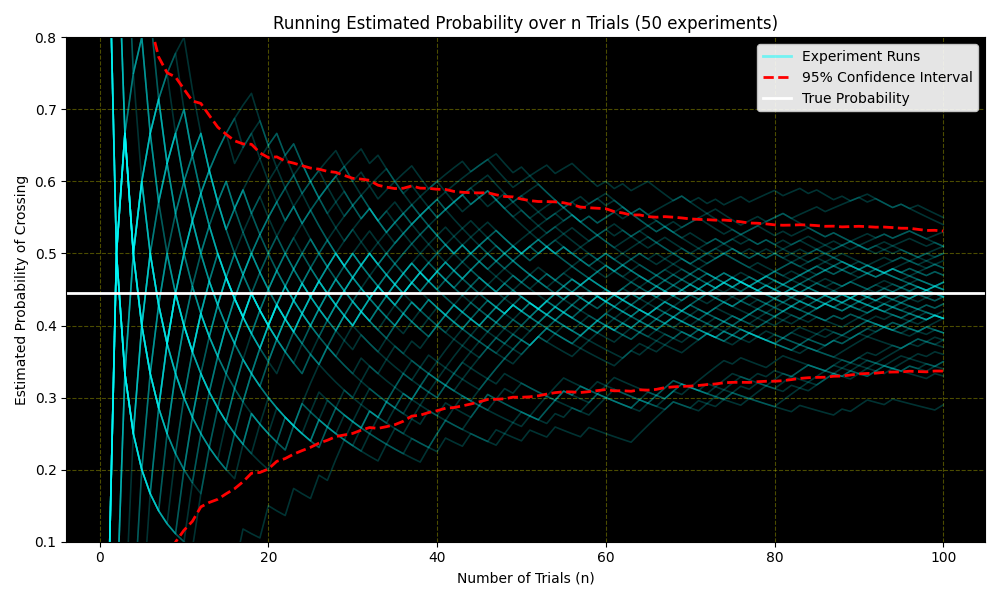
\includegraphics[width=0.7\textwidth]{Task 1/plots/1d_probability_convergence.png}
    \caption{Running probability estimate for 50 independent experiments and
             95\,\% binomial confidence envelope around $P_{\text{true}}$.}
    \label{fig:task1-conv}
\end{figure}

Trajectories fluctuate strongly at small $n$ but concentrate around
$P_{\text{true}} \approx 0.4456$ as $n$ grows.  The CI envelope narrows
visibly with $n$, and the cloud of estimates remains roughly centered on the
true value, suggesting the estimator is unbiased in practice.

\subsection{Subtask e -- Confidence Interval Coverage}

Finally, we measure how often the true probability lies outside the
95\,\% CI as $n$ grows (Figure~\ref{fig:task1-ci}).

\begin{figure}[h]
    \centering
    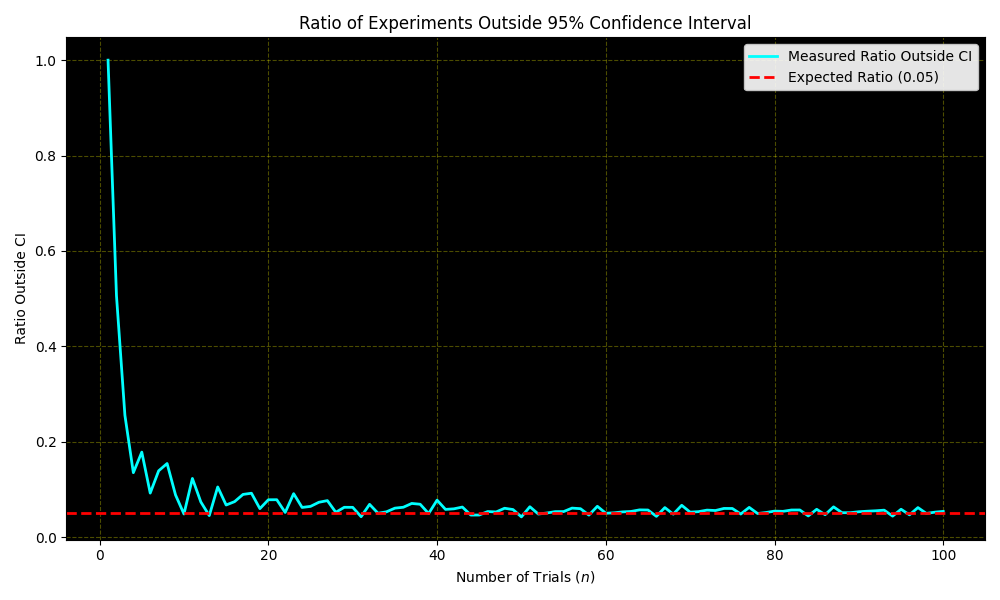
\includegraphics[width=0.7\textwidth]{Task 1/plots/1e_ratio_outside_ci.png}
    \caption{Fraction of experiments in which $P_{\text{true}}$ falls outside
             the 95\,\% CI, plotted against $n$.}
    \label{fig:task1-ci}
\end{figure}

At $n = 1$ the measured outside ratio is very high because the empirical
proportion can only be $0$ or $1$, producing a degenerate interval.  The ratio
drops quickly within the first few trials and then fluctuates around the
expected value of $0.05$.  Small deviations from $0.05$ are due both to the
finite number of repetitions and to the normal approximation used by the
binomial CI, but the asymptotic behavior matches the design coverage of the
interval.

\subsection{Discussion}

The experiment illustrates three Monte Carlo lessons.  First, the number of
trials drives the quality of the estimate, with variance shrinking like
$1/\sqrt{n}$, so early trials yield large precision gains and later ones
yield much smaller ones.  Second, the 95\,\% CI is a statement about
long-run frequency, not about any single experiment: about 5\,\% of
intervals miss the true value, which our coverage experiment confirms once
$n$ is large enough for the normal approximation to be reasonable.  Third,
estimating $\pi$ via Buffon's Needle is indirect -- we measure $P$ and then
invert $\pi = 2L/(DP)$ -- so any error in the measured probability propagates
into the $\pi$ estimate, and stable $\pi$ estimation requires enough trials to
make $\hat P$ reliable.

\newpage
% =============================================================================
\section{Task 2 -- Anti-Agents in Swarm Aggregation}
% =============================================================================

\subsection{Overview}

We extend the baseline swarm-aggregation behavior of Tutorial~2 with
anti-agents, following the swarm-controlled emergence idea of
Scheidler, Merkle and Middendorf (IEEE SIS~2007 / IJICC~2013).  Normal robots
aggregate as before: they wander, stop on neighbor detection, and resume
wandering after a bounded wait.  Anti-agents look like normal
\texttt{foot-bot}s but never stop; they wander continuously, count stopped
neighbors within their sensing range, and broadcast a ``leave'' message
whenever a local cluster exceeds a size threshold.  Stopped normals that
receive a leave order abandon the cluster.  The simulator (ARGoS\,3) and the
analysis toolchain run inside a single Docker image; source, the
\texttt{argos} configuration, both Lua controllers, and the Python scripts
live under \texttt{Task~2/}.

We sweep the anti-agent percentage
$p \in \{0\%, 5\%, 10\%, 15\%, 20\%, 30\%\}$ on a fixed total swarm size of
$30$ robots in a $4 \times 4~$m arena, with $5$ independent repetitions per
setting (each run lasts $200~$s of simulated time).  In total $30$ runs
produced $408{,}000$ log rows analyzed in this section.

\subsection{Implementation}

\paragraph{Normal robot FSM (\texttt{task2.lua}).}
Three states, communicating only via the Range-and-Bearing (RAB) sensor:
\begin{itemize}
    \item \textbf{WANDER} -- forward at \texttt{MAX\_VELOCITY = 20~cm/s} with
          obstacle avoidance.  Transitions to \textbf{STOPPED} when at least
          one other normal robot is within
          \texttt{STOP\_DISTANCE = 25~cm}.  Anti-agents are explicitly ignored
          for this trigger.  LED: green.
    \item \textbf{STOPPED} -- zero velocity; wait timer counts down
          (\texttt{WAIT\_TICKS = 30} = $3.0~$s).  Either the timer expires
          (return to WANDER) or an anti-agent within
          \texttt{ANTI\_RANGE = 60~cm} broadcasts a leave flag -- in the
          latter case the robot enters \textbf{LEAVING}.  LED: red.
    \item \textbf{LEAVING} -- forced wander for $1.0~$s with obstacle
          avoidance active but stop triggers ignored, so the robot actually
          escapes the cluster instead of immediately re-aggregating with the
          same neighbor.  LED: yellow.
\end{itemize}

\paragraph{Anti-agent (\texttt{anti\_agent.lua}).}
The anti-agent has no FSM.  Every tick it counts the number of stopped
normals within \texttt{SCAN\_RANGE = 60~cm} from its RAB messages.  If that
count is $\ge$~\texttt{CLUSTER\_THRESHOLD = 3} it broadcasts a leave order
(LED: magenta), otherwise it stays silent (LED: blue).  This is the
cluster-size dependent disruption rule from the task sheet: small,
``parasitic'' clusters of 1--2 robots are left alone; only larger clusters
are broken up.  Motion is the same obstacle-avoidance random walk, plus a
small per-tick probability of an in-place random reorientation to keep
exploration unbiased.

\paragraph{RAB message layout.}
Each broadcast carries 3 bytes: byte~1 is the agent type ($0$ = normal,
$1$ = anti); byte~2 is the leave flag ($1$ = ``leave the cluster!''); byte~3
is the \texttt{STOPPED} flag (normals only).  This minimal layout lets normals
distinguish each other from anti-agents and lets anti-agents count stopped
normals around them.

\paragraph{Experiment pipeline.}
\texttt{task2.argos} declares the arena, two \texttt{distribute} blocks (one
per role), the foot-bot sensors, and the Lua entry points.
\texttt{run\_experiments.py} patches the two \texttt{entity quantity}
attributes for each $(p,\text{rep})$ pair, strips the visualization block,
fixes a deterministic seed
($\text{seed} = 1000 + 31p + \text{rep}$), runs \texttt{argos3} headlessly,
and parses the per-tick \texttt{DATA} log lines into a tidy CSV
(\texttt{data/all\_runs.csv}).  \texttt{plot\_results.py} consumes the CSV
and produces the four figures and summary tables discussed below.

\subsection{Subtasks a, b -- Local Rule and Bounded Wait}

The baseline aggregation behavior (subtasks a and b of the assignment) is
realized by the WANDER~$\leftrightarrow$~STOPPED loop above.  The local rule
is the RAB-triggered transition at $25~$cm; the bounded wait is the $3.0~$s
timer.  These are the same primitives as in Tutorial~2 -- in this tutorial
they form the substrate that the anti-agents perturb.

\subsection{Subtask c -- Anti-Agents and Swarm-Controlled Emergence}

\paragraph{Aggregation kinetics.}
Figure~\ref{fig:task2-stopped} shows the fraction of normal robots in
the STOPPED state over time, averaged across repetitions, for each
anti-agent percentage.

\begin{figure}[h]
    \centering
    
\includegraphics[width=0.85\textwidth]{Task 2/plots/task2_stopped_over_time.png}
    \caption{Fraction of normal robots in STOPPED state vs.\ simulated time,
             per anti-agent percentage.  The red dashed line marks the
             $80\%$ aggregation threshold used in Table~\ref{tab:task2-ttc}.}
    \label{fig:task2-stopped}
\end{figure}

With $0\%$ anti-agents the swarm jumps to nearly $100\%$ stopped within a
few seconds and stays there.  As $p$ grows the curve sits lower and
oscillates.  No condition prevents the $80\%$
threshold from being reached within $200~$s, but the quality of the
aggregate -- one tight cluster vs.\ many small chains -- differs strongly,
which the next two figures quantify.

\paragraph{Time to reach the aggregation threshold.}
Figure~\ref{fig:task2-ttc} and Table~\ref{tab:task2-ttc} report the first
simulated time at which the stopped fraction reaches $80\%$.

\begin{figure}[h]
    \centering
    
\includegraphics[width=0.7\textwidth]{Task 2/plots/task2_time_to_cluster.png}
    \caption{Time to reach the $80\%$ aggregation threshold vs.\ anti-agent
             percentage.  Markers are means over $5$ repetitions; bars are
             $\pm$~std.}
    \label{fig:task2-ttc}
\end{figure}

\begin{table}[h]
\centering
\begin{tabular}{cc}
\toprule
\textbf{Anti-agent \%} & \textbf{Time to $80\%$ stopped (s)} \\
\midrule
$0\%$   & $7.5 \pm 1.1$  \\
$5\%$   & $12.4 \pm 3.4$ \\
$10\%$  & $12.0 \pm 7.8$ \\
$15\%$  & $12.6 \pm 4.5$ \\
$20\%$  & $15.7 \pm 7.7$ \\
$30\%$  & $16.1 \pm 7.5$ \\
\bottomrule
\end{tabular}
\caption{Mean $\pm$ std time to reach $80\%$ stopped, over $5$ repetitions
         per setting.  No run failed to cross the threshold within $200~$s.}
\label{tab:task2-ttc}
\end{table}

Introducing any anti-agents roughly doubles the time to reach $80\%$
stopped, and the delay grows monotonically with $p$.  The $30$-robot,
$4 \times 4~$m arena is dense enough that aggregation is robust: the
anti-agents delay it but never prevent it within the run budget
(failure fraction $= 0$ for every $p$).

\paragraph{Biggest cluster -- the swarm-controlled-emergence effect.}
The most interesting result is the size of the largest spatial connected
component of stopped normals in the final $20~$s of each run, where two
stopped normals are linked when their Euclidean distance is below
\texttt{CLUSTER\_DIST}~$=0.35~$m (computed via a simple union-find).
Figure~\ref{fig:task2-bc} and Table~\ref{tab:task2-bc} report the result.

\begin{figure}[h]
    \centering
    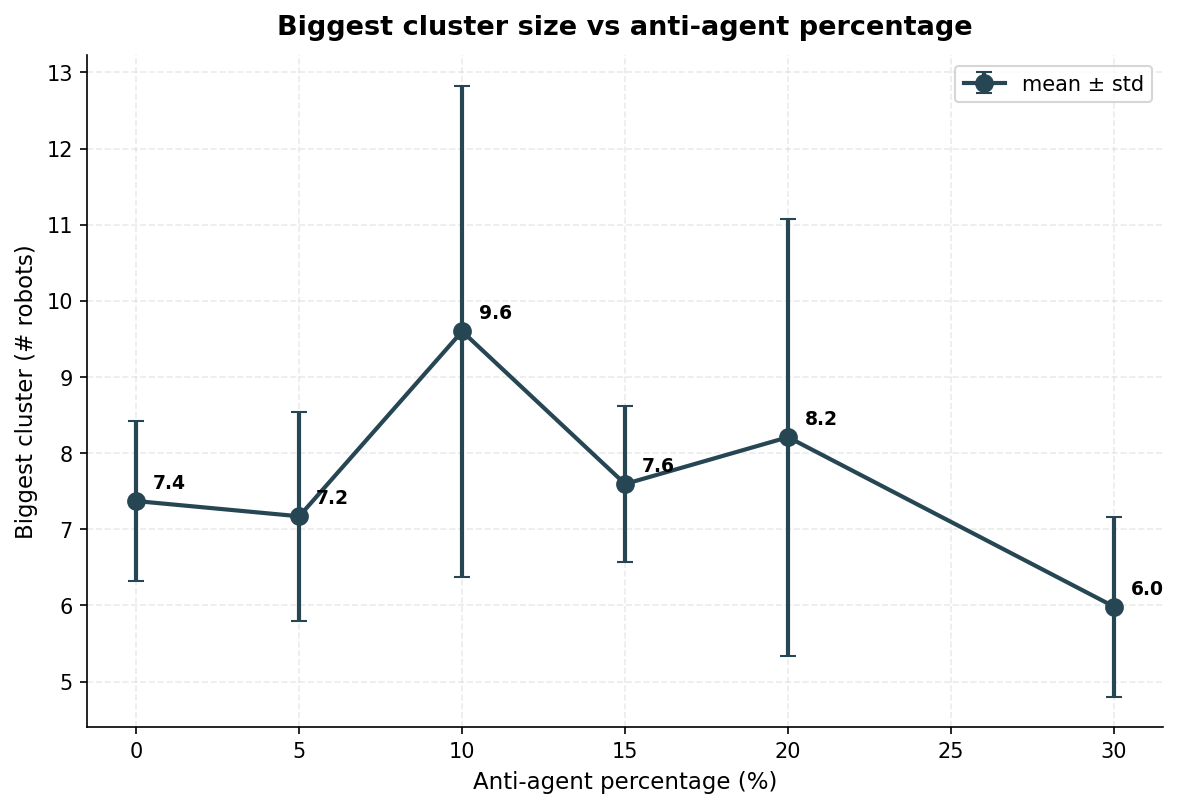
\includegraphics[width=0.7\textwidth]{Task 2/plots/task2_biggest_cluster.png}
    \caption{Mean biggest-cluster size in the final $20~$s vs.\ anti-agent
             percentage.  Error bars show $\pm$~std across $5$ repetitions.}
    \label{fig:task2-bc}
\end{figure}

\begin{table}[h]
\centering
\begin{tabular}{cc}
\toprule
\textbf{Anti-agent \%} & \textbf{Biggest cluster (\# robots)} \\
\midrule
$0\%$           & $7.4 \pm 1.0$ \\
$5\%$           & $7.2 \pm 1.4$ \\
$10\%$          & $9.6 \pm 3.2$ \\
$15\%$          & $7.6 \pm 1.0$ \\
$20\%$          & $8.2 \pm 2.9$ \\
$30\%$          & $6.0 \pm 1.2$ \\
\bottomrule
\end{tabular}
\caption{Mean $\pm$ std biggest-cluster size (number of stopped normals in
         the largest connected component, $0.35~$m link distance, final
         $20~$s of each run).}
\label{tab:task2-bc}
\end{table}

The biggest cluster is non-monotone in the anti-agent percentage.
The $10\%$ setting yields the largest cluster ($9.6$ robots on
average, vs.\ $7.4$ for the unperturbed baseline) -- the counter-intuitive
``anti-agents help clustering'' regime predicted by Scheidler/Merkle.  At
$30\%$ the biggest cluster drops to $6.0$, below baseline: this is the
expected disruptive regime where too many anti-agents prevent the cluster
from consolidating at all.  The variance at the helpful regime is large
($\text{std}\approx 3.2$ over $5$ repetitions), so the effect is not
statistically conclusive at this sample size, but the trend is the one
predicted by the paper and the task sheet's warning that the effect is
``tricky to reproduce'' matches our observation that it only emerges in a
narrow percentage band.

\paragraph{Leave orders per anti-agent.}
Figure~\ref{fig:task2-leave} reports the number of leave orders issued per
anti-agent over the whole run, averaged over repetitions.

\begin{figure}[h]
    \centering
    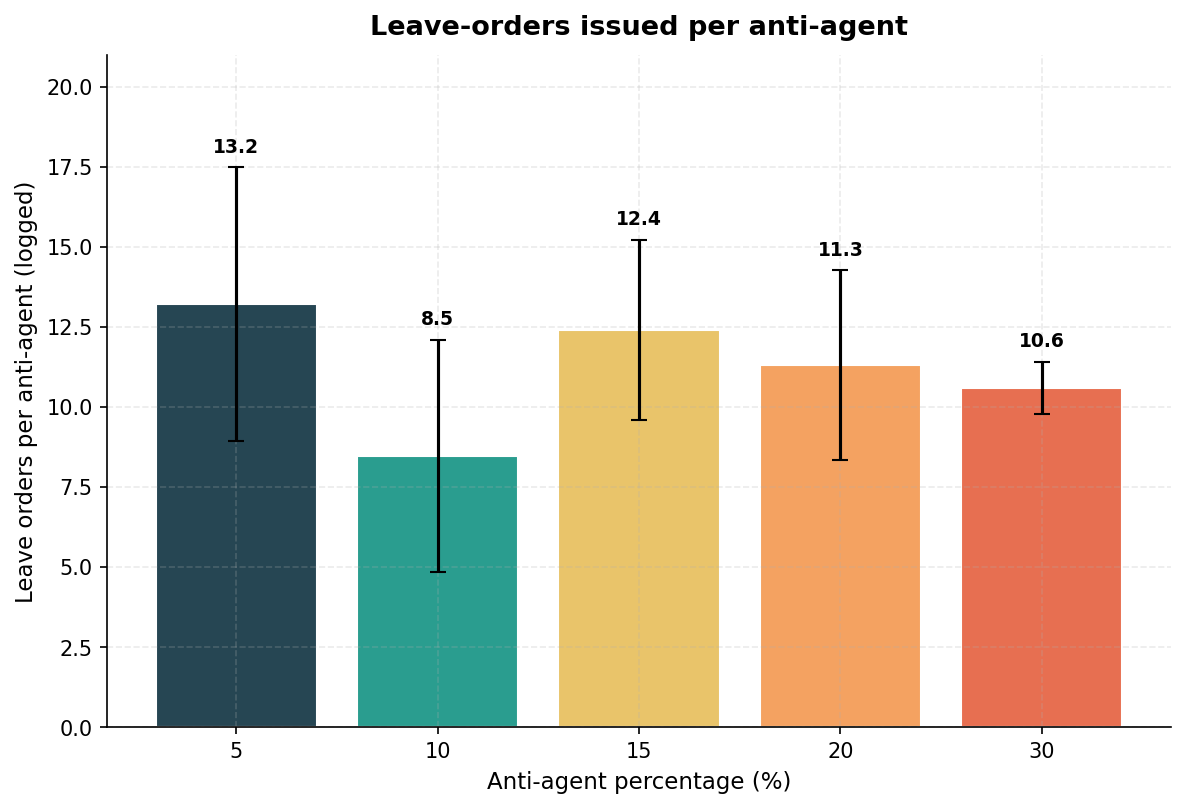
\includegraphics[width=0.7\textwidth]{Task 2/plots/task2_leave_orders.png}
    \caption{Mean leave orders issued per anti-agent vs.\ anti-agent
             percentage.  Bars are $\pm$~std across $5$ repetitions.}
    \label{fig:task2-leave}
\end{figure}

\begin{table}[h]
\centering
\begin{tabular}{cc}
\toprule
\textbf{Anti-agent \%} & \textbf{Leave orders / agent} \\
\midrule
$5\%$           & $13.2 \pm 4.3$ \\
$10\%$          & $8.5 \pm 3.6$ \\
$15\%$          & $12.4 \pm 2.8$ \\
$20\%$          & $11.3 \pm 3.0$ \\
$30\%$          & $10.6 \pm 0.8$ \\
\bottomrule
\end{tabular}
\caption{Mean $\pm$ std number of leave orders issued per anti-agent over
         the $200~$s run.}
\label{tab:task2-leave}
\end{table}

The $10\%$ setting shows the fewest leave orders per anti-agent,
consistent with the biggest-cluster table: when the swarm spends most of
its time in one large, stable cluster, each anti-agent passes through and
out of it quickly without continuously re-triggering the leave condition.
At other percentages the cluster repeatedly fragments and rebuilds, so each
anti-agent finds itself near a cluster more often and broadcasts more.

\clearpage
% =============================================================================
\section{Task 3 -- Local Sampling in a Swarm}
% =============================================================================

\subsection{Overview}

We study a local sampling scenario in a simulated swarm: $N$ robots
are placed uniformly at random in the unit square $[0,1]^2$, each robot is
independently colored black or white with probability $1/2$, and each robot
observes only the colors of robots that fall inside its sensing
neighborhood of radius $r$ (including itself).  From its local observation,
robot $i$ estimates the global number of black robots by scaling its local
black fraction by the swarm size:
\[
    \hat{B}_i \;=\; \frac{B_i^{\text{local}}}{N_i^{\text{local}}} \cdot N.
\]
We sweep $N \in \{2, 4, 6, \ldots, 200\}$ and
$r \in \{0.05,\,0.10,\,0.25,\,0.50\}$, run $1000$ independent experiments per
$(N, r)$ setting, and report two metrics: the mean relative error
of the swarm-average estimate, and the standard deviation of the
individual estimates within the swarm.  Source code lives in
\texttt{Task~3/task\_3.py}.

\subsection{Implementation}

For each experiment, robot positions $(x_i, y_i)$ are drawn from
$\mathcal{U}[0,1]^2$ and colors $c_i \in \{0, 1\}$ from
$\mathcal{U}\{0, 1\}$.  Pairwise distances are computed with
\texttt{scipy.spatial.distance.cdist} and the neighborhood of robot $i$ is
$\{j : d(i, j) < r\}$, which always contains $i$ itself.  Each robot then
forms its estimate $\hat{B}_i$ as above.  For each independent experiment we
record (i) the swarm-average estimate
$\bar{\hat B} = \frac{1}{N}\sum_i \hat B_i$ and its relative error against
the true count $B = \sum_i c_i$, and (ii) the population standard deviation
of the $\hat B_i$.  The reported values are averaged over $1000$ repetitions
per $(N, r)$.

\subsection{Results}

Figure~\ref{fig:task3-results} shows both metrics as a function of swarm size
for the four tested sensor ranges.

\begin{figure}[h]
    \centering
    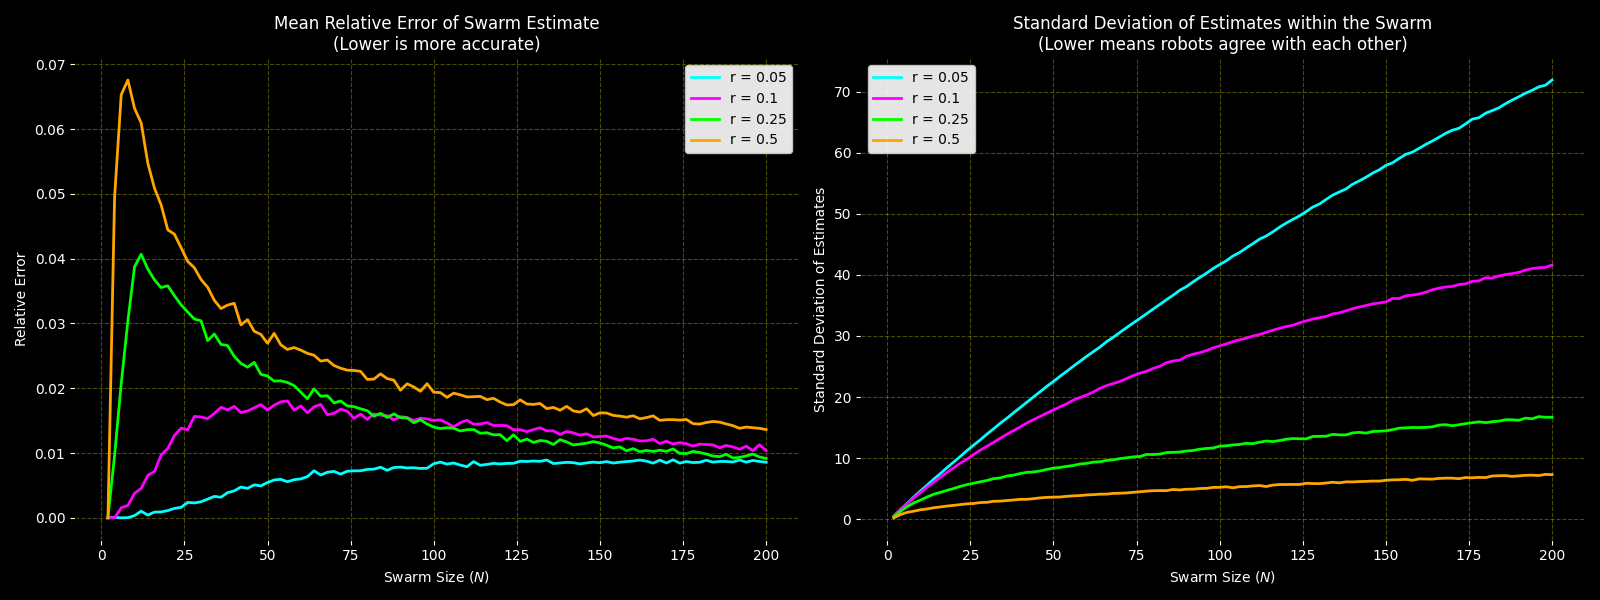
\includegraphics[width=0.95\textwidth]{Task 3/plots/3_mean_error_and_std_vs_n.png}
    \caption{Left: mean relative error of the swarm-average estimate.
             Right: standard deviation of individual robot estimates.
             Both as a function of swarm size $N$, for sensor ranges
             $r \in \{0.05,\,0.10,\,0.25,\,0.50\}$.}
    \label{fig:task3-results}
\end{figure}

\paragraph{Mean relative error.}
For the smallest range $r = 0.05$, the swarm-average error stays low across
the entire $N$ sweep and grows only slightly with $N$.  For larger ranges
($r = 0.25$ and $r = 0.50$) the error is high for small and medium $N$ and
then decreases as $N$ grows; $r = 0.50$ exhibits the most pronounced early
peak (${\sim}0.07$) before relaxing toward ${\sim}0.014$ near $N = 200$.
The intuition is that with a tiny sensing radius most robots see only
themselves or a handful of neighbors and produce extreme estimates close to
$0$ or $N$; these extremes cancel when averaged across the swarm and
the swarm-average happens to recover the global fraction well.  Larger radii
produce more moderate but spatially correlated estimates, and at small $N$
boundary effects and clustering noise bias the average more visibly.

\paragraph{Standard deviation of individual estimates.}
The picture reverses when looking at intra-swarm disagreement.  Smaller
sensor ranges produce by far the largest disagreement -- by $N = 200$ the
standard deviation exceeds $70$ for $r = 0.05$ and stays above $40$ for
$r = 0.10$.  Larger ranges produce much tighter agreement: $r = 0.25$ ends
in the mid-to-high teens, and $r = 0.50$ stays below ${\sim}8$ even at
$N = 200$.  The reason is that larger neighborhoods overlap more across
robots, so different robots draw conclusions from increasingly similar
samples and their estimates converge.  The standard deviation also grows
with $N$ for every $r$, because the estimate $\hat{B}_i$ is scaled by $N$,
so the same relative spread inflates in absolute terms.

\subsection{Discussion}

The two metrics reveal a clear accuracy/agreement trade-off: small
sensor ranges can give a good swarm-average estimate (errors cancel
across the swarm) while simultaneously producing very poor individual
estimates that disagree wildly with each other.  Large sensor ranges produce
worse small-$N$ average accuracy but much better inter-robot agreement.

Which regime is preferable depends on how the swarm uses the estimate.  If
the output is computed centrally by averaging all robots' estimates, even a
very short range can suffice.  If, instead, each robot must act
independently on its own estimate, then short-range sensing leads to
inconsistent decisions across the swarm, and a larger range -- or an
explicit consensus / communication mechanism -- is required.  In practice,
the mean error alone is not a sufficient evaluation metric for a swarm: the
intra-swarm spread of estimates is equally important.

\newpage
% =============================================================================
\section{Completed Tasks}
% =============================================================================

\begin{center}
\begin{tabular}{lll}
\toprule
\textbf{Task} & \textbf{Description} & \textbf{Status} \\
\midrule
1 & Derivation of crossing probability and $\pi$ estimator        & \checkmark \\
1 & Single Buffon's Needle simulation ($n = 1000$)                & \checkmark \\
1 & Standard deviation vs.\ number of trials                      & \checkmark \\
1 & Probability convergence with 95\,\% confidence interval       & \checkmark \\
1 & Confidence interval coverage ratio                            & \checkmark \\
\midrule
2 & Stop on neighbor detection and bounded wait (ARGoS, Lua FSM)  & \checkmark \\
2 & Anti-agent controller with cluster-size-dependent leave rule  & \checkmark \\
2 & Sweep over anti-agent percentage ($30$ runs, $200~$s each)    & \checkmark \\
2 & Kinetics, biggest-cluster, time-to-cluster, leave-order plots & \checkmark \\
2 & Reproduction of Scheidler/Merkle helpful-disruption effect    & \checkmark \\
\midrule
3 & Local sampling: per-robot estimates of global black count     & \checkmark \\
3 & Sweep over swarm size $N$ and sensor range $r$                & \checkmark \\
3 & Mean relative error and intra-swarm estimate spread analysis  & \checkmark \\
\bottomrule
\end{tabular}
\end{center}

\end{document}
